\documentclass[uplatex,a4j]{jsarticle}
\usepackage[top=35truemm,bottom=30truemm,left=30truemm,right=30truemm]{geometry}
%フォント設定
%\usepackage[deluxe,jis2004]{otf}
\usepackage{amsmath}
\usepackage{amsfonts}
\usepackage{bm}
\usepackage[dvipdfmx]{graphicx}
\usepackage[dvipdfmx]{color}
\usepackage{listings,jlisting}
\usepackage{amsmath,amssymb}
\usepackage{latexsym}
\usepackage{url}
%\usepackage{xcolor}
\usepackage{here}

\providecommand{\tabularnewline}{\\}
\newcommand{\argmax}{\mathop{\rm argmax}\limits}
\newcommand{\argmin}{\mathop{\rm argmin}\limits}

\lstset{
  %language=bash,
 	%枠外に行った時の自動改行
 	breaklines = true,
 	%自動改行後のインデント量(デフォルトでは20[pt])
 	breakindent = 10pt,
 	%標準の書体
 	basicstyle = \ttfamily\scriptsize,
 	%コメントの書体
 	commentstyle = {\itshape \color[cmyk]{1,0.4,1,0}},
 	%関数名等の色の設定
 	classoffset = 0,
 	%キーワード(int, ifなど)の書体
 	keywordstyle = {\bfseries \color[cmyk]{0,1,0,0}},
 	%表示する文字の書体
 	stringstyle = {\ttfamily \color[rgb]{0,0,1}},
 	%枠 "t"は上に線を記載, "T"は上に二重線を記載
	%他オプション:leftline,topline,bottomline,lines,single,shadowbox
 	frame = tbrl,
 	%frameまでの間隔(行番号とプログラムの間)
 	framesep = 5pt,
 	%行番号の位置
 	numbers = left,
	%行番号の間隔
 	stepnumber = 1,
	%行番号の書体
 	numberstyle = \tiny,
	%タブの大きさ
 	tabsize = 4,
 	%キャプションの場所("tb"ならば上下両方に記載)
 	captionpos = b
}

\title{新人課題}
\author{津嶋 佑旗}
\date{\today}

\begin{document}
  \maketitle
  \section{配列情報処理}
  \subsection{ヒト21番染色体の先頭コンティグのDNA配列を秋山研サーバから取得し,A/T/G/Cの各塩基数を出力せよ.}
  以下のように実行する.実行環境はPython2で,ghostgw上での動作を確認している.
  \begin{lstlisting}[caption=実行方法, label=run1]
    python 1_1.py /mnt/fs/ohue/newcomer/NT_113952.1.fasta
  \end{lstlisting}
  プログラム本体は{\tt 1\_1.py}である.fastaファイルの塩基配列について,行ごとにPythonの機能で各文字の出現回数をカウントする.
  実行した結果が以下の通りである.
  \lstinputlisting[caption=実行結果, label=result1]{./result_1_1.txt}
  
  \subsection{NT\_113952.1.fastaの逆相補鎖を生成するプログラムを作成せよ.}
  以下のように実行する.実行環境はPython2で,ghostgw上での動作を確認している.
  \begin{lstlisting}[caption=実行方法, label=run2]
    python 1_2.py /mnt/fs/ohue/newcomer/NT_113952.1.fasta
  \end{lstlisting}
  プログラム本体は{\tt 1\_2.py}と{\tt rev.py},{\tt combine.py}である.
  実行結果はresult\_1\_2.txtとして別添する.
  
  \subsection{ウィンドウ幅$w$,ステップ幅$s$で,ウィンドウ内のGC含量を出力するプログラムを作成し,NT\_113952.1.fastaに$w=1000$,$s=300$で適用した結果をgnuplot等Excel以外のツールでプロットせよ.}
  以下のように実行する.実行環境はPython2で,ghostgw上での動作を確認している.
  \begin{lstlisting}[caption=実行方法, label=run3]
    python 1_3.py /mnt/fs/ohue/newcomer/NT_113952.1.fasta 1000 300 > data.txt
  \end{lstlisting}
  プログラム本体は{\tt 1\_3.py}である.また,{\tt combine.py}も使用する.
  実行結果をgnuplotで描画した結果以下のようになった.
  \begin{figure}[htbp]
    \begin{center}
      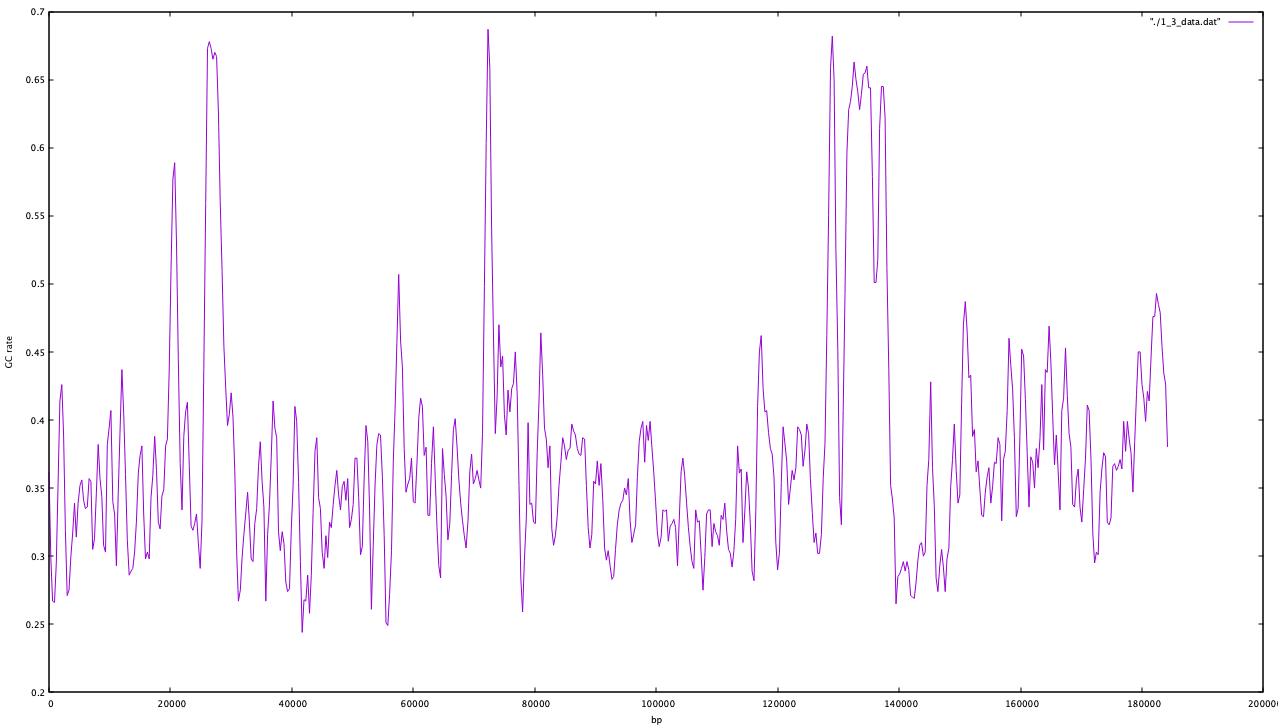
\includegraphics[width=15cm]{1_3_plot.png}
      \caption{グラフ}
    \end{center}
  \end{figure}
  
  \subsection{引数で与えられた部分配列を検索し,何文字目に現れたかを表示するプログラムを作成せよ(逆相補鎖上も検索すること).部分配列をGAATTCおよびATGとし,NT\_113952.1.fastaに適用せよ.}
  以下のように実行する.実行環境はPython2で,ghostgw上での動作を確認している.
  \begin{lstlisting}[caption=実行方法, label=run4]
    python 1_4.py /mnt/fs/ohue/newcomer/NT_113952.1.fasta GAATTC
    python 1_4.py /mnt/fs/ohue/newcomer/NT_113952.1.fasta ATG
  \end{lstlisting}
  プログラム本体は{\tt 1\_4.py}と{\tt findall.py}である.また,{\tt rev.py}と{\tt combine.py}も使用する.
  実行した結果が以下の通りである.ただし,ATGの結果については極端に長いためresult\_1\_4\_ATG.txtとして別添する.
  \lstinputlisting[caption=実行結果(GAATTC), label=result4]{./result_1_4_GAATTC.txt}
  
  \subsection{NT\_113952.1.fastaを6つの読み枠でアミノ酸配列に変換せよ.Stopコドンはアンダースコアで表示すること.}
  以下のように実行する.実行環境はPython2で,ghostgw上での動作を確認している.
  \begin{lstlisting}[caption=実行方法, label=run5]
    python 1_5.py /mnt/fs/ohue/newcomer/NT_113952.1.fasta
  \end{lstlisting}
  プログラム本体は{\tt 1\_5.py}と{\tt decode.py}である.また,{\tt rev.py}と{\tt combine.py}も使用する.
  実行した結果が以下の通りである.
  \lstinputlisting[caption=実行結果, label=result5]{./result_1_5.txt}
  
  \section{タンパク質構造情報処理}
  \subsection{PyMOLソフトウェアを利用し,ヒトのヘモグロビンの構造をチェインごとに異なる色で表示し,4量体であることを確認せよ.また,Aチェインだけを表示し,タンパク質鎖をcartoon表示して2次構造に従って色付けし,結合するヘムをstick表示して原子ごとに色分けせよ.}
  チェインごとに色分けしたヘモグロビンが画像\ref{2_6_1}である.
  \begin{figure}[H]
    \begin{center}
      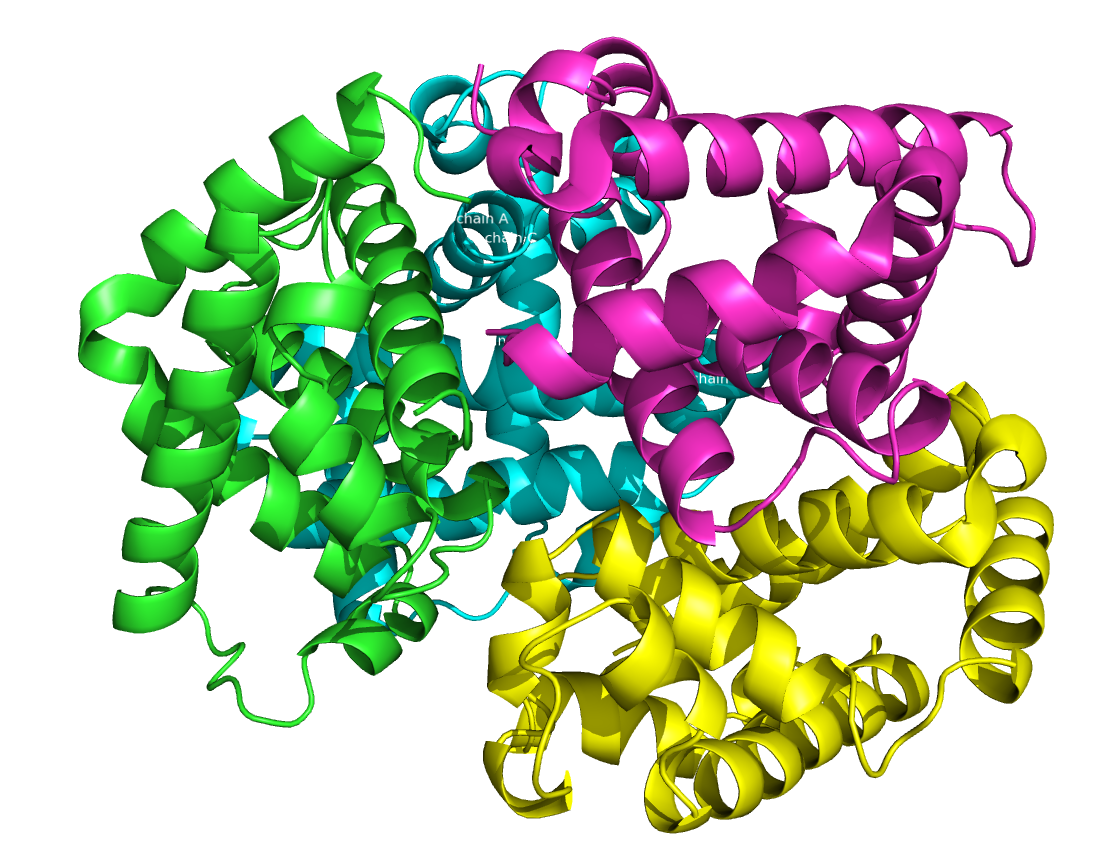
\includegraphics[width=12cm]{1BUW.png}
      \caption{ヘモグロビン}
      \label{2_6_1}
    \end{center}
  \end{figure}
  また,Aチェインとヘムを表示したものが画像\ref{2_6_2}である.
  \begin{figure}[H]
    \begin{center}
      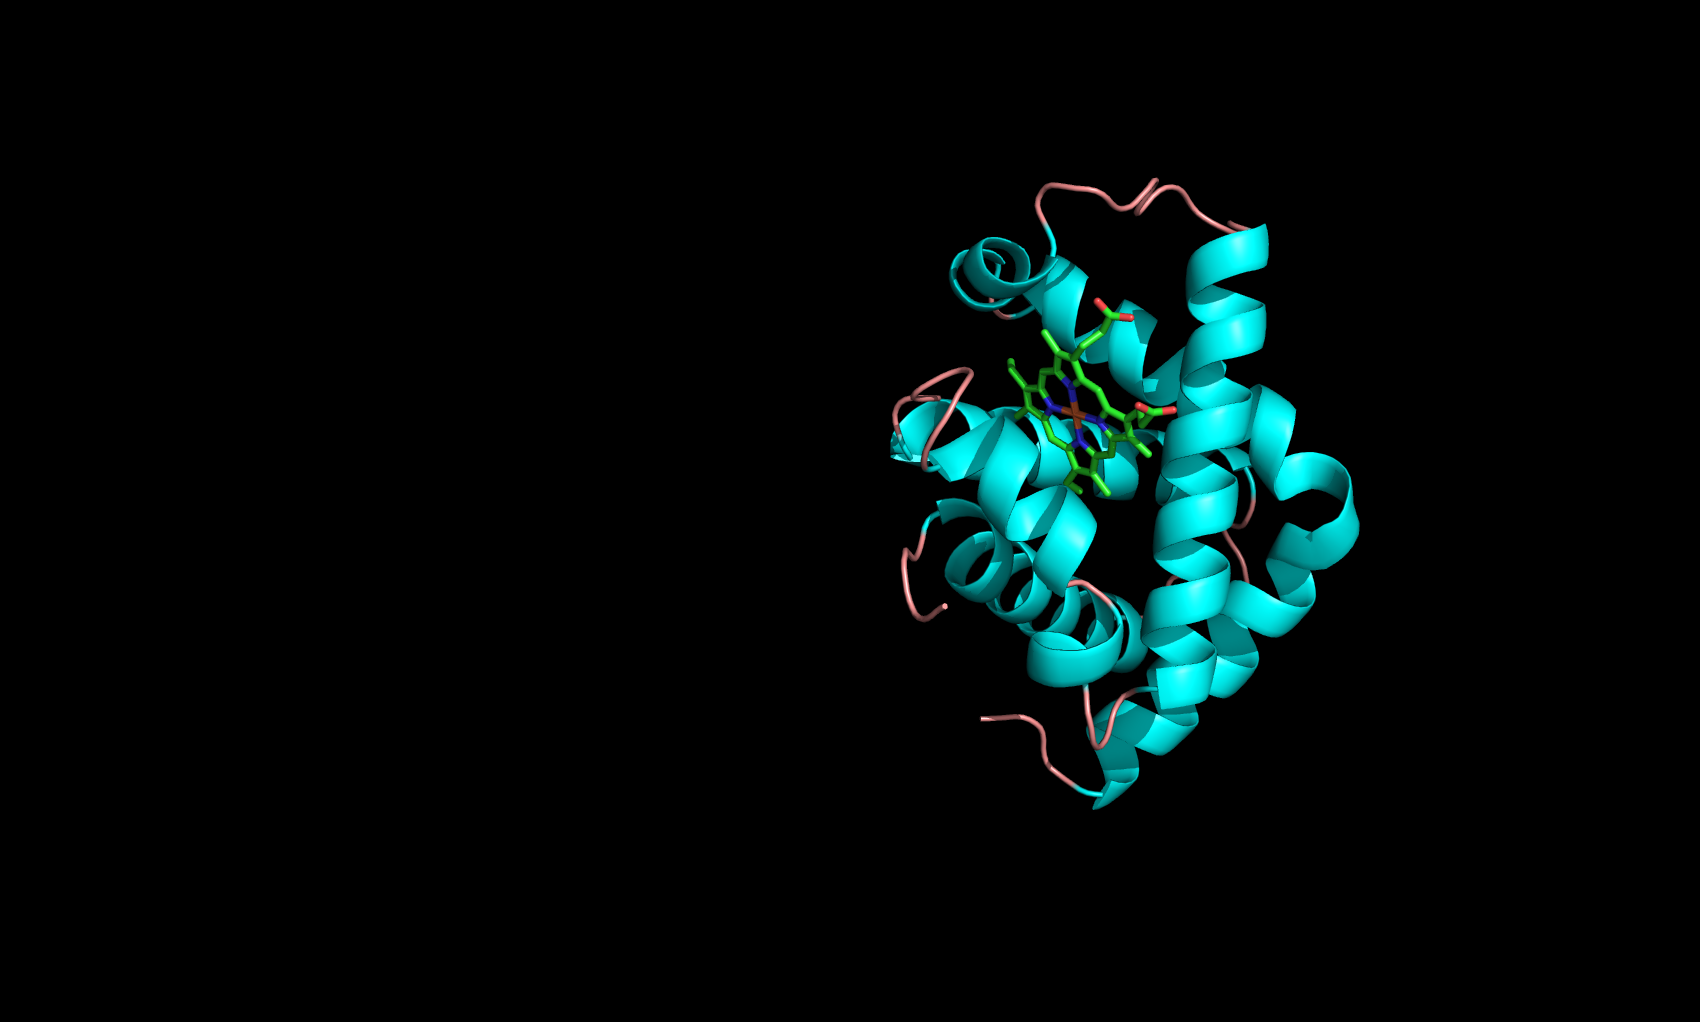
\includegraphics[width=12cm]{hem.png}
      \caption{Aチェインとヘム}
      \label{2_6_2}
    \end{center}
  \end{figure}
  
  \subsection{PDBファイル名とチェイン名を引数にして,その回転半径を計算するプログラムを作成せよ.}
  \subsection{上記のプログラムの結果を利用し,PyMOLで重心から回転半径の範囲内にある原子を赤で,範囲外にある原子を青で色付けせよ.}
  この2つは一緒に行い,プログラム{\tt 2\_7.py}を作成した.実行環境はAnaconda3のPython 2.7環境である.
  このプログラムを次のように実行する.
  \begin{lstlisting}[caption=実行方法, label=run6]
    python 2_7.py ./1BUW.pdb A
  \end{lstlisting}
  結果は次の通りである.
  \lstinputlisting[caption=実行結果, label=result6]{./result_2_7.txt}
  また,描画結果として以下の画像を得た.
  \begin{figure}[H]
    \begin{center}
      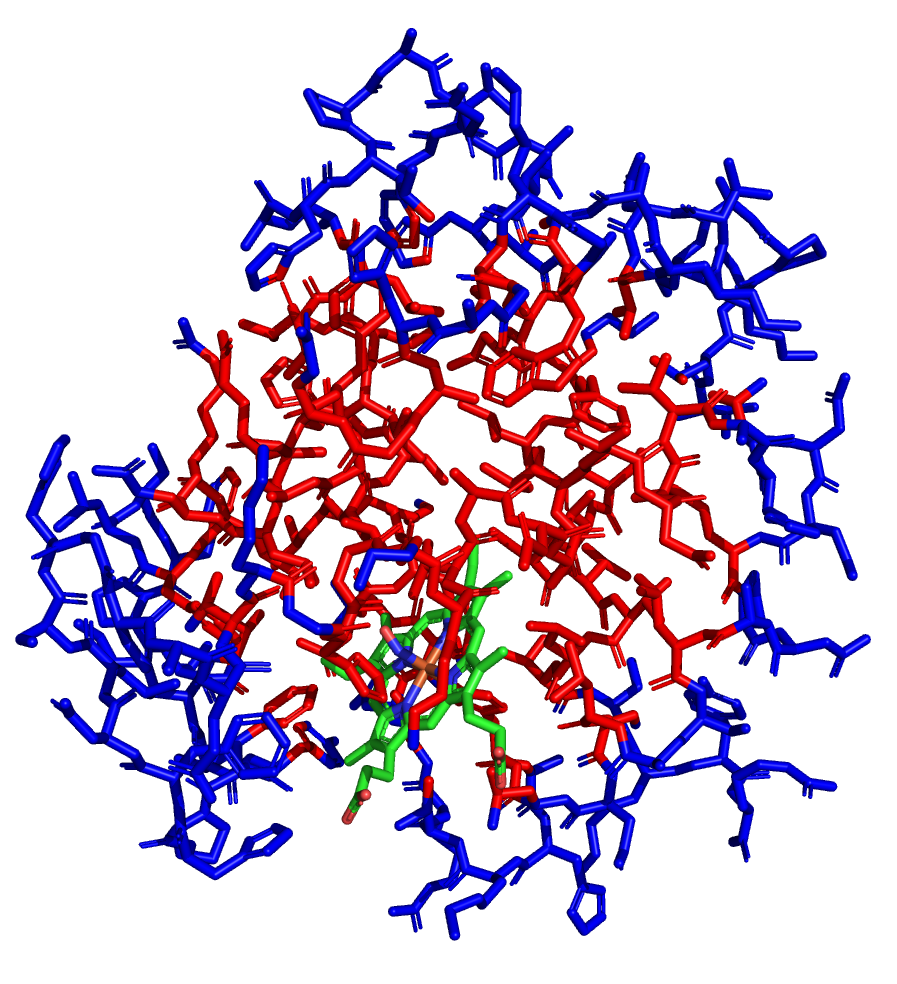
\includegraphics[width=12cm]{2_8.png}
      \caption{回転半径}
      \label{2_8}
    \end{center}
  \end{figure}
  
  \section{機械学習}
  \subsection{Pythonのscikit-learnのSVMでionosphereのデータの10-fold Cross Validationを実施せよ.予測性能としてprecision,recall,MCC,ROC曲線のAUC値(AUROC),F-scoreを求めよ.カーネルはRBFカーネルとし,パラメータは適宜定めよ.}
  プログラム{\tt 3\_9.py}を作成した.Anaconda3のPython2.7環境で動作する.
  また,ionosphere.scaleの読み込みにあたって,欠番のパラメータを0で補完するなどの処理を行うため,読み込み部分は別のプログラム{\tt load\_ionosphere.py}として分離した.
  実行した結果を\ref{result7}に示す.
  \lstinputlisting[caption=実行結果, label=result7]{./result_3_9.txt}
  
  \subsection{ionosphereデータにおいて,より良いRBFカーネルパラメータ$\gamma$とコストパラメータ$C$の値を探索せよ.評価方法は10-fold Cross Validationとし,評価基準はAUROCとF-scoreの2通りを試すこと.}
  プログラム{\tt 3\_10.py}を作成した.Anaconda3のPython2.7環境で動作する.
  実行した結果を\ref{result9}に示す.
  \lstinputlisting[caption=実行結果, label=result9]{./result_3_10.txt}
  
  \section{創薬情報処理・機械学習}
  \subsection{(準備1)PythonにRDKitをインストールし,化合物ファイル(SDFファイル)を読み込んで構造式が出力できることを確認せよ.}
  省略する.
  
  \subsection{(準備2)論文Leung SSF, et al. J Chem Inf Model 56: 924-020, 2016.のSupporting Informationより,3D SDFファイル(TXT)とPDFファイルをダウンロードせよ.Table S1の実験値「RRCK Log P$_\text{app}$」の値をパース(転記)し,CSVファイル等で準備せよ.}
  省略する.
  
  \subsection{(準備3)所望の化合物に対し,RDKitのECFP4 fingerprintを計算できるようにせよ.}
  calc\_fgprint関数を作成した.コードは{\tt calc\_fgprint.py}の通りである.
  
  \subsection{RRCK Log P$_\text{app}$を目的関数,ECFP4 fingerprintを特徴ベクトルとして,Data Set 3(医薬品104化合物)に関して回帰(10-fold Cross Validation)を行う機械学習プログラムを作成せよ.学習器はSupport Vector Regressionとし,カーネルはRBFカーネルとすること.}
  スクリプト{\tt 4\_14.py}を作成した.
  実行結果は\ref{result414}の通りである.
  \lstinputlisting[caption=実行結果, label=result414]{./result_4_14.txt}
  
  \subsection{10-fold Cross Validationによって,RRCK Log P$_\text{app}$の予測値との平均2乗誤差(RMSE)が最も小さくなるパラメータを探索せよ.またそのときのRMSEと$R^2$値を求めよ.}
  スクリプト{\tt 4\_15.py}を作成した.
  実行結果は\ref{result415}の通りである.
  \lstinputlisting[caption=実行結果, label=result415]{./result_4_15.txt}
  
  \subsection{(15)で決めたパラメータの学習器で,Data Set 1(環状ペプチド7化合物),Data Set 4(環状ペプチド16化合物),Data Set 8(環状ペプチド22化合物)のRRCK Log P$_\text{app}$の予測値を求めよ.それぞれのData SetごとにRMSEと$R^2$値を求め,予測値と実験値の散布図を描け.}
  スクリプト{\tt 4\_16.py}を作成した.
  実行結果は\ref{result416}の通りである.
  \lstinputlisting[caption=実行結果, label=result416]{./result_4_16.txt}
  また,実験値と予測値の散布図は出力したファイルからGnuplotで描画した.図\ref{1},\ref{3},\ref{4},\ref{8}を得た.
  \begin{figure}[H]
    \begin{center}
      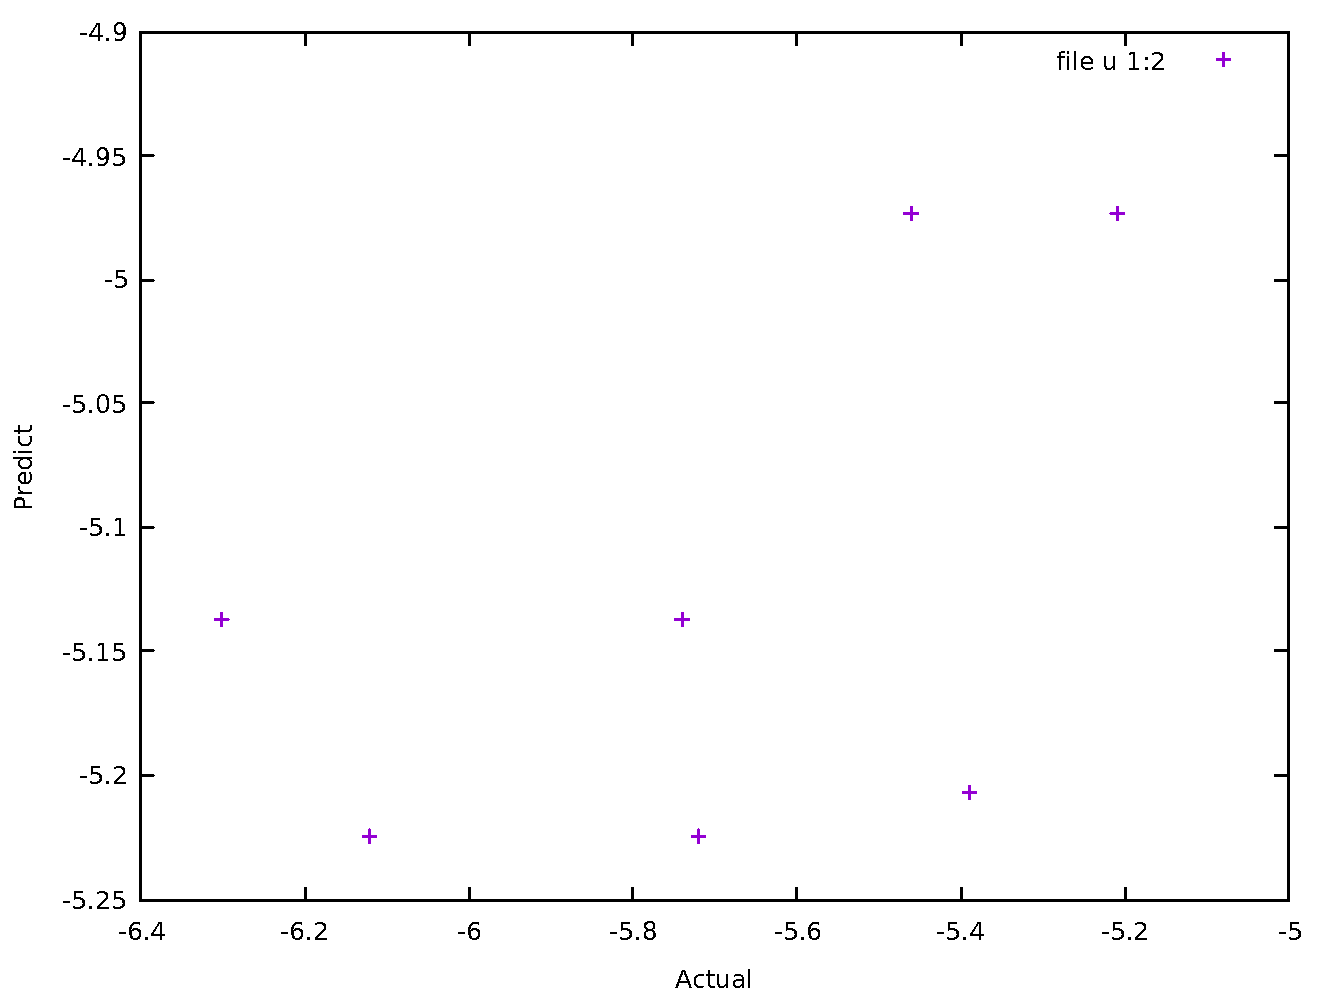
\includegraphics[width=13cm]{pre1.pdf}
      \caption{Data Set 1}
      \label{1}
    \end{center}
  \end{figure}
  \begin{figure}[H]
    \begin{center}
      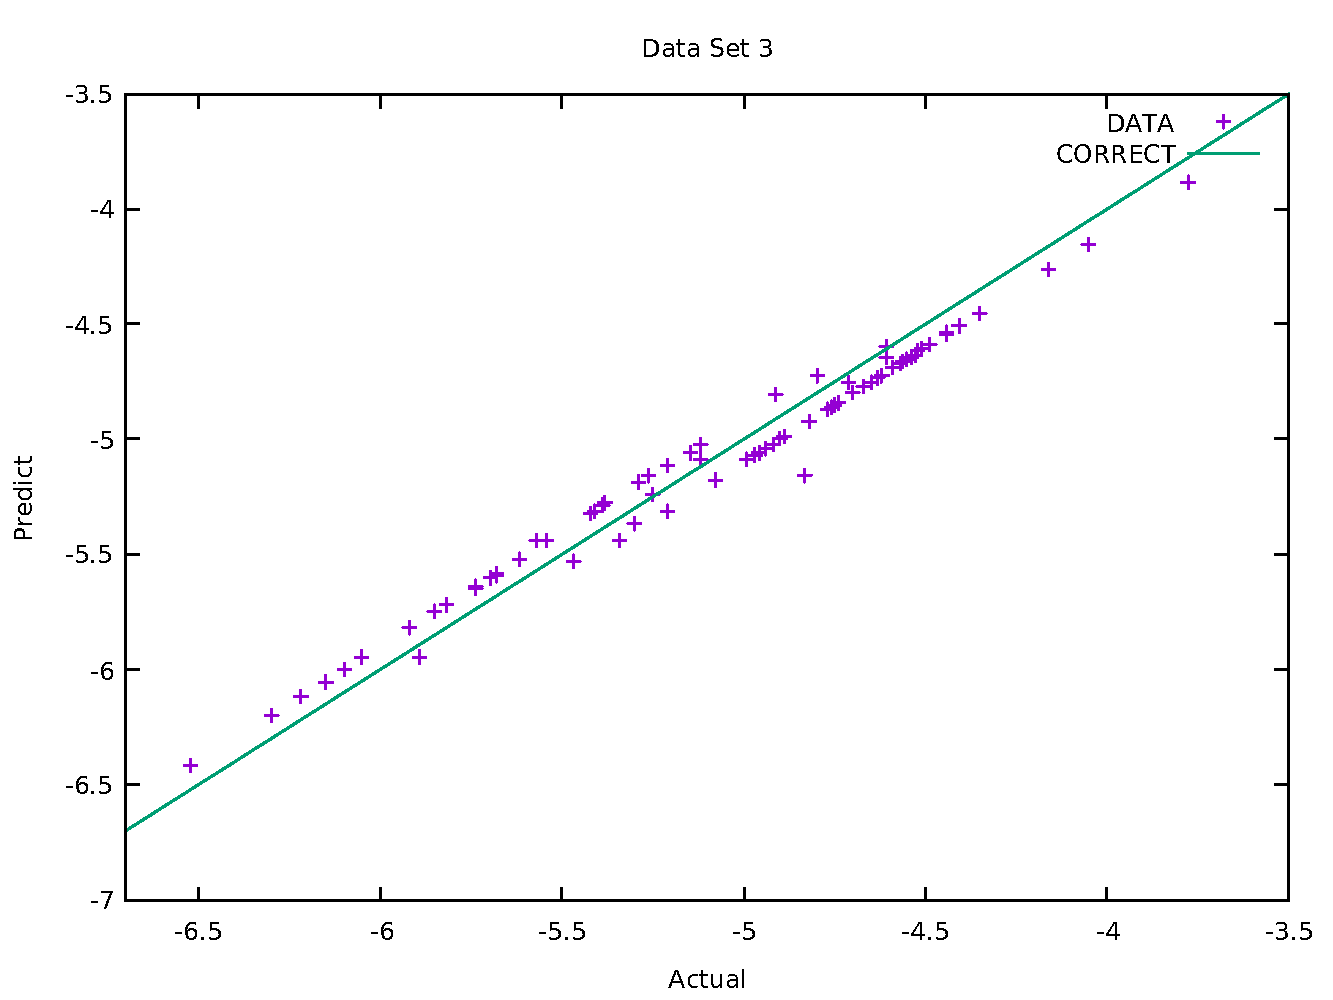
\includegraphics[width=13cm]{pre3.pdf}
      \caption{Data Set 3}
      \label{3}
    \end{center}
  \end{figure}
  \begin{figure}[H]
    \begin{center}
      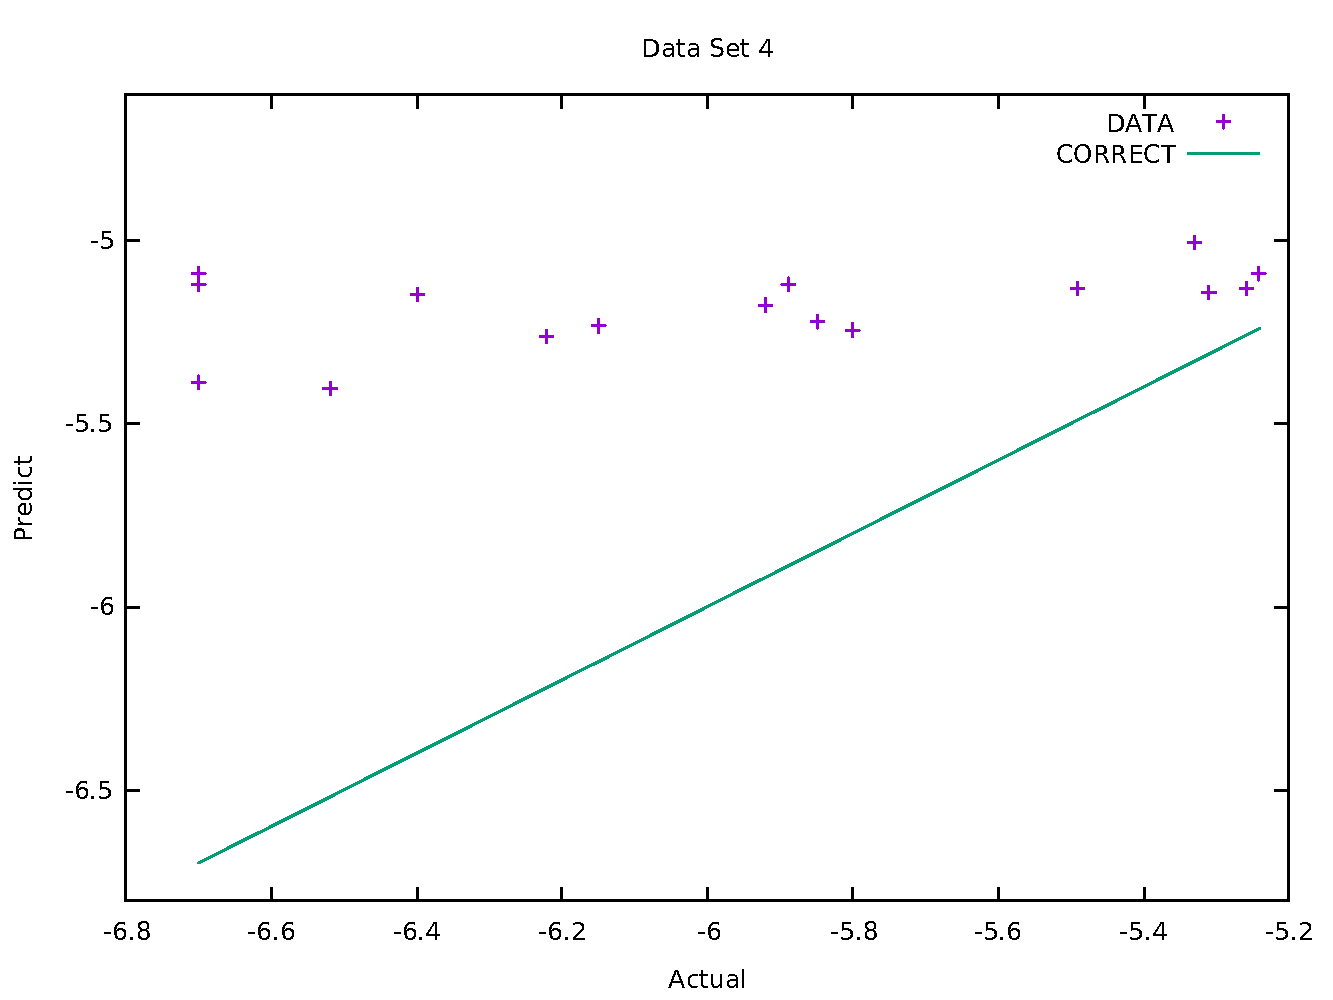
\includegraphics[width=13cm]{pre4.pdf}
      \caption{Data Set 4}
      \label{4}
    \end{center}
  \end{figure}
  \begin{figure}[H]
    \begin{center}
      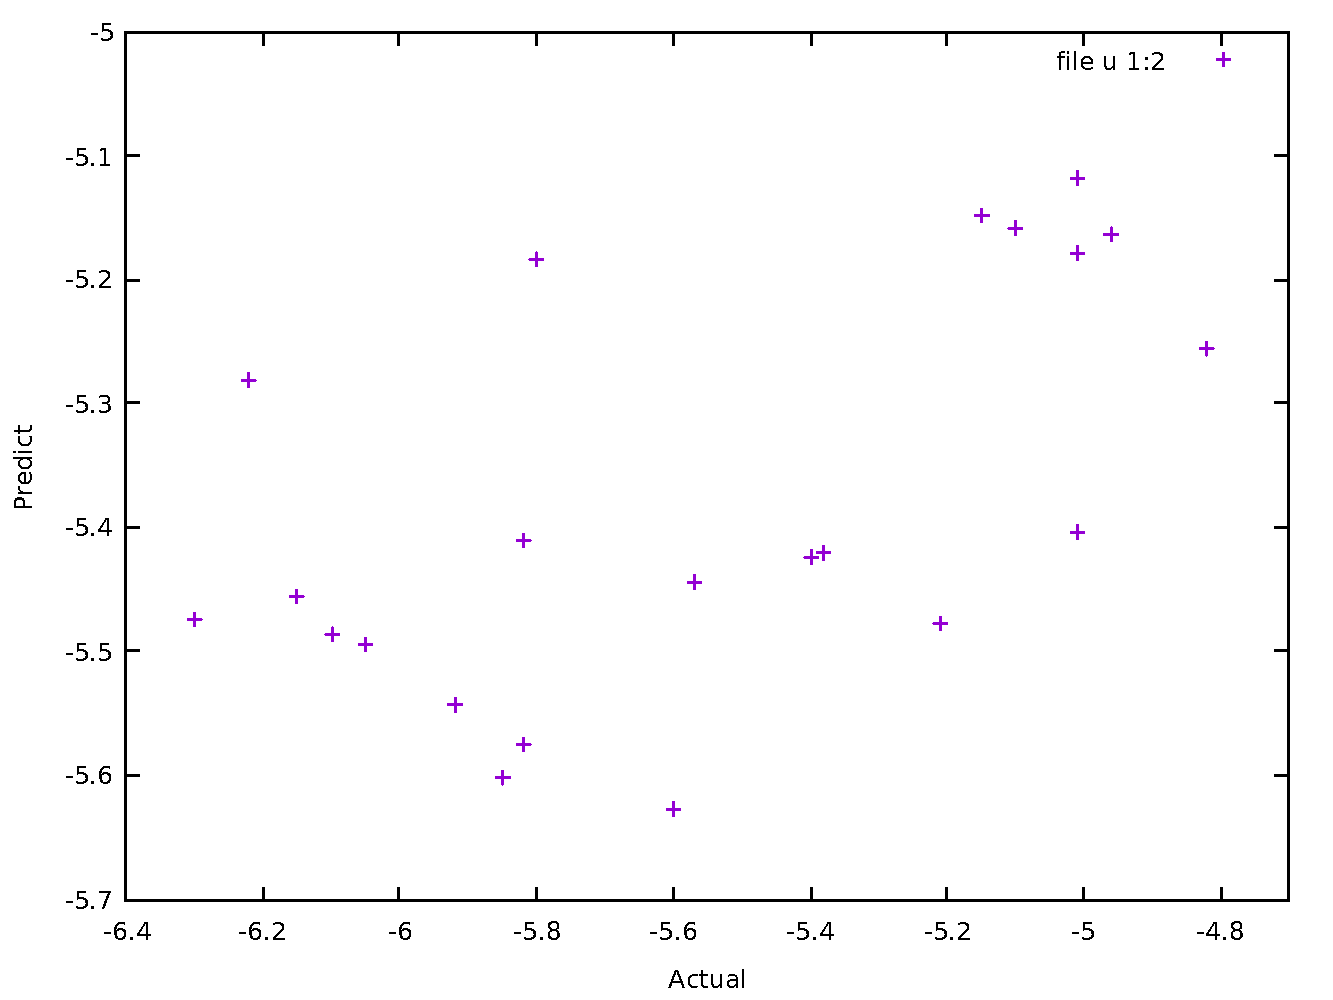
\includegraphics[width=13cm]{pre8.pdf}
      \caption{Data Set 8}
      \label{8}
    \end{center}
  \end{figure}
  
\end{document}
